\documentclass[conference]{IEEEtran}
\IEEEoverridecommandlockouts
\usepackage{cite}
\usepackage{amsmath,amssymb}
\usepackage{graphicx}
\usepackage{booktabs}
\usepackage{multirow}
\usepackage{url}
\usepackage{tikz}
\usepackage{pgfplots}
\pgfplotsset{compat=1.18}
\usetikzlibrary{arrows.meta,positioning}

\begin{document}

\title{Extractive or Generative? Small Local Language Models for Evidence-Grounded Pharmacovigilance Question Answering}

\author{\IEEEauthorblockN{Akhil Mahadik}
\IEEEauthorblockA{\textit{Information Technology} \\
\textit{Vidyalankar Institute of Technology}\\
Mumbai, India \\
akhil.mahadik@vit.edu.in}
\and
\IEEEauthorblockN{Diyansh Jain}
\IEEEauthorblockA{\textit{Information Technology} \\
\textit{Vidyalankar Institute of Technology}\\
Mumbai, India \\
diyansh.jain@vit.edu.in}
}

\maketitle

\begin{abstract}
Retrieval-augmented generation (RAG) is attractive for drug-safety question answering, but privacy and cost often require small language models that run on local hardware, and a fluent wrong answer about a drug's safety is worse than no answer. We built a local pharmacovigilance assistant over the U.S.\ FDA Adverse Event Reporting System (FAERS, 2025 Q1) and an evidence corpus of FDA drug labels, FDA Drug Safety Communications and PubMed reviews (601 documents, 8{,}590 passages), and compared extractive answering with generation by three small instruction-tuned models (Qwen2.5-0.5B, Qwen2.5-1.5B, SmolLM2-1.7B) on a single 4\,GB laptop GPU. All systems saw identical retrieved passages; ground truth came from FDA's own label section coding, so no item was hand-labelled. On a factual safety check (\emph{``Does drug X have a boxed warning?''}, 89 held-out drugs) the extractive answer was correct for 92.1\% of drugs, against 43.8\%, 69.7\% and 49.4\% for the generators (all $p<10^{-4}$, exact McNemar). A citation-and-support verifier accepted 51--52\% of generated drafts, yet 16--47\% of accepted drafts were wrong; the dominant errors were polarity biases that lexical verification cannot see (Qwen2.5-1.5B denied 23 of 45 existing boxed warnings; SmolLM2-1.7B asserted one for all 44 drugs without). Allowing verified generations into the answer therefore \emph{lowered} accuracy for both Qwen models (to 74.2\% and 76.4\%). Generation helped only for choosing which passage answers a lay question, where Qwen2.5-1.5B with verification outperformed extractive top-1 selection (77.5\% vs 67.4\%, $p=0.012$). For factual safety claims with small local models, extractive answering is the safer default; generation is best confined to passage selection and presentation.
\end{abstract}

\begin{IEEEkeywords}
pharmacovigilance, retrieval-augmented generation, small language models, faithfulness, abstention, drug labels, FAERS
\end{IEEEkeywords}

\section{Introduction}
Post-marketing drug safety relies on spontaneous adverse-event reports. Disproportionality statistics such as the reporting odds ratio (ROR) and proportional reporting ratio (PRR) flag drug--reaction pairs that are reported together more often than expected \cite{evans2001prr,vanpuijenbroek2002ror,noren2013shrinkage}, but such signals are hypotheses, not evidence of causation \cite{hauben2009signal}. A user asking \emph{``Does Ozempic cause pancreatitis?''} needs both what the reports show and what established sources---drug labelling and the literature---state, clearly kept apart.

Retrieval-augmented generation (RAG) \cite{lewis2020rag} conditions a language model on retrieved passages and is a natural fit. Generated text, however, can be unfaithful to its sources \cite{maynez2020faithfulness,ji2023hallucination}, and attributing statements to evidence remains difficult even for large models \cite{gao2023alce,rashkin2023ais}. In many health settings, data-protection rules, cost or connectivity rule out hosted large models, leaving \emph{small} models on local hardware. Whether such models add value over simply quoting the retrieved evidence is an empirical question with safety consequences.

We study this question in a working system and make four contributions:
\begin{enumerate}
\item A fully local RAG pipeline that joins FAERS statistics computed in DuckDB with FDA labels, FDA Drug Safety Communications and PubMed reviews, separates \emph{observed reports} from \emph{established evidence}, and declines when evidence is insufficient.
\item A label-free evaluation protocol that uses FDA's structured product labeling (SPL) section coding as ground truth for retrieval and answering.
\item A controlled, paired comparison of extractive answering against three small generators (0.5--1.7B parameters) under identical retrieval, with a citation-and-support verifier.
\item Evidence that verification of this kind is necessary but not sufficient: it rejects unsupported text but passes confident polarity errors, so generation lowered accuracy on a factual safety task while helping on passage selection.
\end{enumerate}

\section{Related Work}
\textbf{RAG and faithfulness.} RAG combines a retriever with a generator \cite{lewis2020rag}. Abstractive generation frequently introduces content unsupported by its input \cite{maynez2020faithfulness}; a broad survey of such hallucinations is given in \cite{ji2023hallucination}. Citation-generating systems \cite{gao2023alce} and attribution metrics \cite{rashkin2023ais} evaluate whether statements are supported by cited sources, typically with large models or human/NLI judgments. We examine the small-model regime with a lightweight lexical verifier.

\textbf{Retrieval.} BM25 \cite{robertson2009bm25} remains a strong lexical baseline; dense sentence encoders such as BGE \cite{xiao2023cpack} capture paraphrase; reciprocal-rank fusion \cite{cormack2009rrf} combines rankers. Biomedical encoders include PubMedBERT \cite{gu2021pubmedbert} and SapBERT for entity linking \cite{liu2021sapbert}.

\textbf{Abstention.} Selective prediction trades coverage for accuracy \cite{geifman2017selective}, and question-answering benchmarks include unanswerable questions to test it \cite{rajpurkar2018squad2}.

\textbf{Pharmacovigilance data.} FAERS is distributed as quarterly extracts \cite{fda2025faers}; openFDA exposes drug labels and other FDA data through an API \cite{kasshout2016openfda}.

\section{System}
\subsection{Observed reports: FAERS statistics}
The 2025 Q1 FAERS extract (400{,}514 reports) was de-duplicated following FDA's case-version rules, giving an analysis population of 392{,}729 cases; ROR, PRR and the information component were computed for 241{,}675 drug--reaction pairs with at least three reports. These statistics are retrieved from DuckDB unchanged and are never produced by a language model. Drug names in a question are matched against the FAERS vocabulary and brand aliases learnt from FAERS; reaction phrases are linked to MedDRA preferred terms with SapBERT \cite{liu2021sapbert}.

\subsection{Established evidence corpus}
For the 150 most-reported suspect drugs we collected (Table~\ref{tab:corpus}): openFDA SPL sections of the manufacturer's most-revised label set, selected via NLM DailyMed; up to four PubMed reviews or meta-analyses on adverse effects published since 2015; and the FDA Drug Safety Communications linked from fda.gov. Labels are chunked \emph{within} SPL sections (160 words, 30-word overlap), so every passage carries its section, document version, date and URL. Passages were embedded with BGE-small-en-v1.5 (384 dimensions) \cite{xiao2023cpack} and searched by exact cosine similarity.

\begin{table}[t]
\caption{Evidence corpus (snapshot of 20 October 2026)}
\label{tab:corpus}
\centering
\begin{tabular}{lrr}
\toprule
Source & Documents & Passages \\
\midrule
FDA drug labels (openFDA SPL) & 135 & 7{,}100 \\
PubMed reviews / meta-analyses & 424 & 759 \\
FDA Drug Safety Communications & 42 & 731 \\
\midrule
Total & 601 & 8{,}590 \\
\bottomrule
\end{tabular}
\end{table}

\subsection{Answering}
For a question, passages are retrieved within the linked drug's sources; if the best cosine similarity is below a calibrated threshold, the system declines. Otherwise the answer is produced in one of two ways (Fig.~\ref{fig:pipeline}).

\emph{Extractive.} A deterministic check reports whether the drug's label mentions the linked reaction term and in which sections; the answer then quotes the best-matching sentence of each top passage verbatim, with its source details.

\emph{Generative.} A small instruction-tuned model receives the top three passages, each tagged with an identifier, source title and SPL section, plus a system prompt and one worked example; it must write two or three sentences, each ending with a passage identifier. Decoding is greedy (at most 160 new tokens), fp16 on the GPU.

\emph{Verifier.} A draft is shown only if (i) it cites at least one passage and only existing identifiers, (ii) every number it contains occurs in the passages, (iii) every quotation is verbatim, and (iv) each sentence shares at least half of its content words (after stemming and removal of reporting verbs) with the passages it cites. Otherwise the extractive answer is shown.

\begin{figure}[t]
\centering
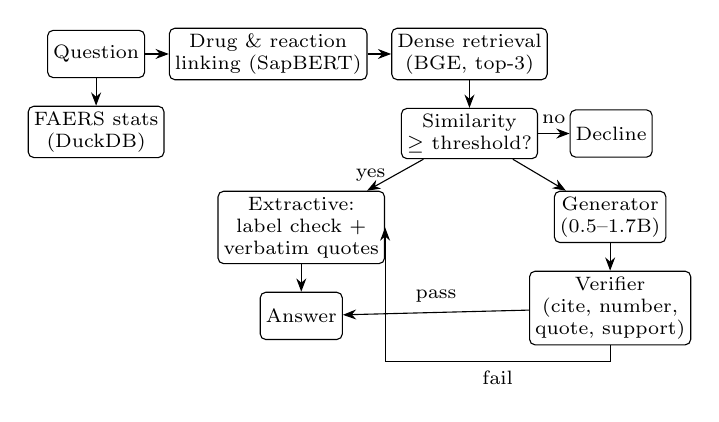
\begin{tikzpicture}[node distance=3.5mm and 3mm, every node/.style={font=\scriptsize, align=center},
  box/.style={draw, rounded corners=2pt, minimum height=6mm, inner sep=2pt}, >=Stealth]
\node[box] (q) {Question};
\node[box, right=of q] (link) {Drug \& reaction\\linking (SapBERT)};
\node[box, right=of link] (ret) {Dense retrieval\\(BGE, top-3)};
\node[box, below=of ret] (suff) {Similarity\\$\geq$ threshold?};
\node[box, below left=4mm and 2mm of suff] (ext) {Extractive:\\label check +\\verbatim quotes};
\node[box, below right=4mm and 2mm of suff] (gen) {Generator\\(0.5--1.7B)};
\node[box, below=of gen] (ver) {Verifier\\(cite, number,\\quote, support)};
\node[box, below=of q] (faers) {FAERS stats\\(DuckDB)};
\node[box, right=4mm of suff] (dec) {Decline};
\node[box, below=of ext] (out) {Answer};
\draw[->] (q) -- (link); \draw[->] (link) -- (ret); \draw[->] (ret) -- (suff);
\draw[->] (suff) -- node[left]{yes} (ext); \draw[->] (suff) -- (gen); \draw[->] (gen) -- (ver);
\draw[->] (ver) -- node[above]{pass} (out); \draw[->] (ext) -- (out);
\draw[->] (q) -- (faers); \draw[->] (suff) -- node[above]{no} (dec);
\draw[->] (ver.south) |- ++(0,-2mm) -| node[pos=0.25, below]{fail} (ext.east);
\end{tikzpicture}
\caption{Answering pipeline. FAERS statistics and external evidence are reported separately; generated drafts are shown only after verification.}
\label{fig:pipeline}
\end{figure}

\section{Evaluation Method}
\subsection{Ground truth from label structure}
FDA codes every label passage by SPL section (Boxed Warning, Contraindications, Drug Interactions, \dots). We use this coding as ground truth, so no item was labelled by the authors or by a model. The 127 drugs with an indexed label were split, with a fixed seed, into 38 development and 89 test drugs; the retriever and abstention threshold were chosen on development drugs only; the prompt and verifier were fixed during system development, before this comparison was run, using a handful of drugs that were not excluded from the test set. All reported results use the 89 test drugs.

\subsection{Retrieval and abstention}
For each drug and each label topic present, a question was posed in label wording (\emph{``What are the contraindications of X?''}) and in lay wording (\emph{``Who should not take X?''}); a hit is relevant if it comes from that drug's gold section. The production retriever was selected on development drugs by mean reciprocal rank (MRR). The abstention threshold was chosen on development drugs to maximise balanced accuracy between answerable questions and templated unanswerable ones (price, packaging colour, unrelated topics).

\subsection{Extractive versus generative answering}
Retrieval was run once and cached, so every system saw identical passages (top three).

\emph{Task A (factual check)}: \emph{``Does X have a boxed warning?''} for all 89 test drugs (45 with, 44 without a Boxed Warning section). The extractive answer is ``yes'' iff a retrieved passage comes from the Boxed Warning section. Generated answers were mapped to yes/no/undetermined with fixed patterns; undetermined counts as wrong.

\emph{Task B (passage selection)}: one lay question per drug on a randomly drawn topic (contraindications 18, pregnancy 24, adverse reactions 20, overdosage 16, interactions 11). The extractive answer is correct iff its first passage is from a gold section; a generated answer is correct iff it cites at least one passage and every cited passage is from a gold section. Task B therefore measures \emph{attribution}, not the clinical content of the answer.

For each model we report raw accuracy, verifier pass rate, accuracy of verified answers, and \emph{system} accuracy---what users would see: the generated answer if verified, otherwise the extractive one. Systems are compared on the same items with the two-sided exact McNemar test; intervals are Wilson 95\%.

\emph{Models}: Qwen2.5-0.5B-Instruct and Qwen2.5-1.5B-Instruct \cite{qwen2024qwen25} (one family, two sizes) and SmolLM2-1.7B-Instruct \cite{allal2025smollm2} (a second family), all Apache-2.0, run on an NVIDIA GeForce RTX 3050 Laptop GPU (4\,GB).

\section{Results}
\subsection{Retrieval and abstention}
Dense retrieval clearly outperformed BM25 and hybrid fusion (Table~\ref{tab:retrieval}); the gap is largest for lay questions, which share few words with label text. Fusion lowered dense performance, and dense retrieval was chosen on development drugs (MRR 0.850 vs 0.752 hybrid and 0.588 BM25). The abstention threshold (cosine 0.73) answered 93.3\% of answerable and declined 91.6\% of unanswerable test questions (balanced accuracy 92.5\%).

\begin{table}[t]
\caption{Finding FDA's gold label section (89 test drugs, 886 questions, search within the drug)}
\label{tab:retrieval}
\centering
\begin{tabular}{lccc}
\toprule
 & Dense & Hybrid (RRF) & BM25 \\
\midrule
Top-1, all questions & \textbf{81.2\%} & 67.2\% & 51.0\% \\
Top-5, all questions & \textbf{94.6\%} & 85.6\% & 70.5\% \\
Top-1, lay wording & \textbf{67.7\%} & 39.5\% & 18.5\% \\
Top-1, label wording & 94.6\% & \textbf{94.8\%} & 83.5\% \\
MRR, all questions & \textbf{0.871} & 0.750 & 0.595 \\
\bottomrule
\end{tabular}
\end{table}

\subsection{Task A: factual safety check}
The extractive answer was correct for 82 of 89 drugs (92.1\%, 95\% CI 84.6--96.1\%); its seven errors were all boxed warnings that retrieval did not surface. Every generator was significantly worse (Table~\ref{tab:taskA}, Fig.~\ref{fig:acc}). Scale helped within a family (Qwen 0.5B$\to$1.5B: 43.8\% $\to$ 69.7\%, McNemar $p=0.002$), but the larger SmolLM2 model was worse than Qwen2.5-1.5B ($p=0.033$).

Crucially, the verifier did not separate right from wrong answers. About half of all drafts passed it, but only 53.3\%, 58.7\% and 84.4\% of accepted drafts were correct. As a result, using verified generations made the system \emph{less} accurate than extractive answering alone for both Qwen models (74.2\%, $p=1.4\times10^{-4}$; 76.4\%, $p=0.003$); for SmolLM2 the drop to 87.6\% was not significant ($p=0.34$).

\begin{table}[t]
\caption{Task A, ``Does X have a boxed warning?'' (89 test drugs). $p$: exact McNemar vs extractive on the same items}
\label{tab:taskA}
\centering
\setlength{\tabcolsep}{3.2pt}
\resizebox{\columnwidth}{!}{%
\begin{tabular}{lcccc}
\toprule
 & Extractive & Qwen 0.5B & Qwen 1.5B & SmolLM2 1.7B \\
\midrule
Raw accuracy & \textbf{92.1\%} & 43.8\% & 69.7\% & 49.4\% \\
\quad 95\% CI & 84.6--96.1 & 34.0--54.2 & 59.5--78.2 & 39.3--59.6 \\
\quad $p$ vs extractive & -- & $1.6{\times}10^{-11}$ & $8.8{\times}10^{-5}$ & $3.2{\times}10^{-8}$ \\
Verifier pass rate & -- & 50.6\% & 51.7\% & 50.6\% \\
Accuracy if verified & -- & 53.3\% & 58.7\% & 84.4\% \\
System accuracy & \textbf{92.1\%} & 74.2\% & 76.4\% & 87.6\% \\
\quad $p$ vs extractive & -- & $1.4{\times}10^{-4}$ & 0.003 & 0.34 \\
\bottomrule
\end{tabular}%
}
\end{table}

\subsection{Why verification fails: polarity errors}
Table~\ref{tab:polarity} shows the errors are systematic. Qwen2.5-1.5B answered ``no'' for 23 of the 45 drugs that \emph{have} a boxed warning, e.g.\ \emph{``No, there is no boxed warning for Capecitabine [L1]''}; 16 of these false negatives passed verification, because the sentence shares the words \emph{boxed}, \emph{warning} and the drug name with its cited passage. SmolLM2-1.7B answered ``yes'' for every drug, including all 44 without a boxed warning; its high accuracy among verified answers reflects this yes-bias meeting a 45:44 class balance, not discrimination. Qwen2.5-0.5B mostly did not answer the question (42 undetermined drafts). A lexical support test cannot detect a flipped polarity; for safety, a verified false ``no boxed warning'' is the most dangerous error.

\begin{table}[t]
\caption{Task A predictions by gold label, and verified wrong answers}
\label{tab:polarity}
\centering
\setlength{\tabcolsep}{3.5pt}
\resizebox{\columnwidth}{!}{%
\begin{tabular}{lccc}
\toprule
 & Qwen 0.5B & Qwen 1.5B & SmolLM2 1.7B \\
\midrule
Has warning (45): yes / no / undet. & 32 / 1 / 12 & 22 / 23 / 0 & 44 / 0 / 1 \\
No warning (44): yes / no / undet. & 7 / 7 / 30 & 4 / 40 / 0 & 44 / 0 / 0 \\
Verified false negatives & 1 & 16 & 0 \\
Verified false positives & 2 & 3 & 7 \\
\bottomrule
\end{tabular}%
}
\end{table}

\begin{figure}[t]
\centering
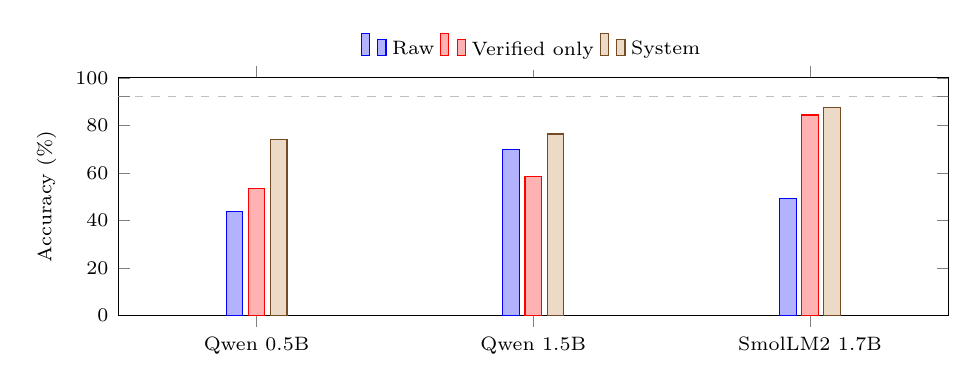
\begin{tikzpicture}
\begin{axis}[ybar, bar width=6pt, width=\columnwidth, height=4.6cm, ymin=0, ymax=100,
  ylabel={Accuracy (\%)}, symbolic x coords={Q0.5,Q1.5,S1.7}, xtick=data,
  xticklabels={Qwen 0.5B, Qwen 1.5B, SmolLM2 1.7B}, ticklabel style={font=\scriptsize},
  label style={font=\scriptsize}, legend style={font=\scriptsize, at={(0.5,1.03)}, anchor=south, legend columns=3, draw=none},
  enlarge x limits=0.25, extra y ticks={92.1}, extra y tick labels={}, extra y tick style={grid=major, major grid style={dashed}}]
\addplot coordinates {(Q0.5,43.8) (Q1.5,69.7) (S1.7,49.4)};
\addplot coordinates {(Q0.5,53.3) (Q1.5,58.7) (S1.7,84.4)};
\addplot coordinates {(Q0.5,74.2) (Q1.5,76.4) (S1.7,87.6)};
\legend{Raw, Verified only, System}
\end{axis}
\end{tikzpicture}
\caption{Task A accuracy by model. The dashed line is extractive answering (92.1\%); no generator configuration reaches it.}
\label{fig:acc}
\end{figure}

\subsection{Task B: passage selection}
For lay questions the picture differs (Table~\ref{tab:taskB}). Extractive top-1 selection cited a gold-section passage for 67.4\% of drugs. Qwen2.5-1.5B cited only gold passages in 71.9\% of answers ($p=0.45$ vs extractive) and passed verification for 68.5\%; with fallback, system accuracy rose to 77.5\%, a significant gain ($p=0.012$; 10 items improved, 1 worsened). The model acts as a re-ranker over the three retrieved passages, gaining most on drug-interaction questions (8/11 vs 4/11). The other models did not help: Qwen2.5-0.5B reached 38.2\% raw and SmolLM2 11.2\% (frequently omitting citations), with system accuracy statistically indistinguishable from extractive. Because Task B scores attribution only, a verified answer can be correctly attributed yet uninformative (e.g.\ \emph{``None of the passages mention who should not take Humira [L1]''}).

\begin{table}[t]
\caption{Task B, lay question per drug: cited passages from the gold label section (89 test drugs)}
\label{tab:taskB}
\centering
\setlength{\tabcolsep}{3.2pt}
\resizebox{\columnwidth}{!}{%
\begin{tabular}{lcccc}
\toprule
 & Extractive & Qwen 0.5B & Qwen 1.5B & SmolLM2 1.7B \\
\midrule
Raw accuracy & 67.4\% & 38.2\% & 71.9\% & 11.2\% \\
\quad $p$ vs extractive & -- & $1.3{\times}10^{-5}$ & 0.45 & $2.4{\times}10^{-14}$ \\
Verifier pass rate & -- & 37.1\% & 68.5\% & 18.0\% \\
Accuracy if verified & -- & 69.7\% & 85.2\% & 37.5\% \\
System accuracy & 67.4\% & 70.8\% & \textbf{77.5\%} & 64.0\% \\
\quad $p$ vs extractive & -- & 0.38 & \textbf{0.012} & 0.38 \\
\bottomrule
\end{tabular}%
}
\end{table}

\subsection{Cost}
Peak GPU memory was 1.1, 3.1 and 3.6\,GB and throughput 33.0, 20.5 and 22.9 tokens/s for the 0.5B, 1.5B and 1.7B models; median time per answer was 0.7--3.3\,s. All fit a 4\,GB laptop GPU in fp16. The extractive answer needs no generator and responds in about 0.1\,s after retrieval.

\section{Discussion}
\textbf{Extractive answering is the safer default for factual safety claims.} On a question with a verifiable yes/no answer, no small generator came close to quoting the retrieved label, and adding verified generations made the system worse. A pilot with Qwen2.5-0.5B on 40 drugs, using hybrid retrieval and four passages, showed the same pattern (35\% vs 97.5\%).

\textbf{Verification is necessary but not sufficient.} The verifier removed drafts without citations, invented numbers or misquotes (in the pilot it also blocked an unsupported claim that metformin should be avoided in pregnancy), but word-overlap support is blind to negation. Errors were systematic biases---denying or asserting a warning regardless of evidence---rather than random noise, so they pass any test that looks only at shared vocabulary. Polarity-aware checks, such as entailment models, deterministic cross-checks against document structure, or answer-type constraints, are needed before generated safety claims can be shown.

\textbf{Generation can help where it selects rather than asserts.} On lay questions, Qwen2.5-1.5B improved attribution by choosing among retrieved passages, a role in which an error is visible (the cited passage is shown) rather than hidden in fluent prose.

\textbf{Model family matters as much as size.} SmolLM2-1.7B was larger than Qwen2.5-1.5B but worse on both tasks, mainly through format non-compliance and a uniform ``yes'' answer.

\textbf{Limitations.} One FAERS quarter and 150 drugs; three models from two families, all below 2B parameters; templated questions rather than real user queries; one factual task with a binary answer; ground truth at the level of label sections, so Task B measures attribution, not clinical correctness; and pattern-based mapping of generated text to yes/no. The evidence corpus is a snapshot and covers PubMed abstracts only.

\section{Conclusion}
In a local pharmacovigilance RAG system, extractive answering over well-retrieved FDA label passages was more accurate than generation by small language models on a factual safety question, and a citation-and-support verifier could not prevent confident polarity errors from reaching the answer. Small generators were useful only for selecting which passage answers a lay question. We recommend that local drug-safety assistants state factual safety claims extractively, reserve small generators for selection and presentation, and adopt polarity-aware verification before allowing generated claims. Future work will evaluate larger local models, entailment-based verification and real user questions with expert-judged answers.

\bibliographystyle{IEEEtran}
\bibliography{refs}

\end{document}
